\section{Referencia de la Clase Cliente\-View}
\label{classClienteView}\index{ClienteView@{ClienteView}}
Muestra la ficha de un cliente.  


{\tt \#include $<$clienteview.h$>$}

Diagrama de herencias de Cliente\-View\begin{figure}[H]
\begin{center}
\leavevmode
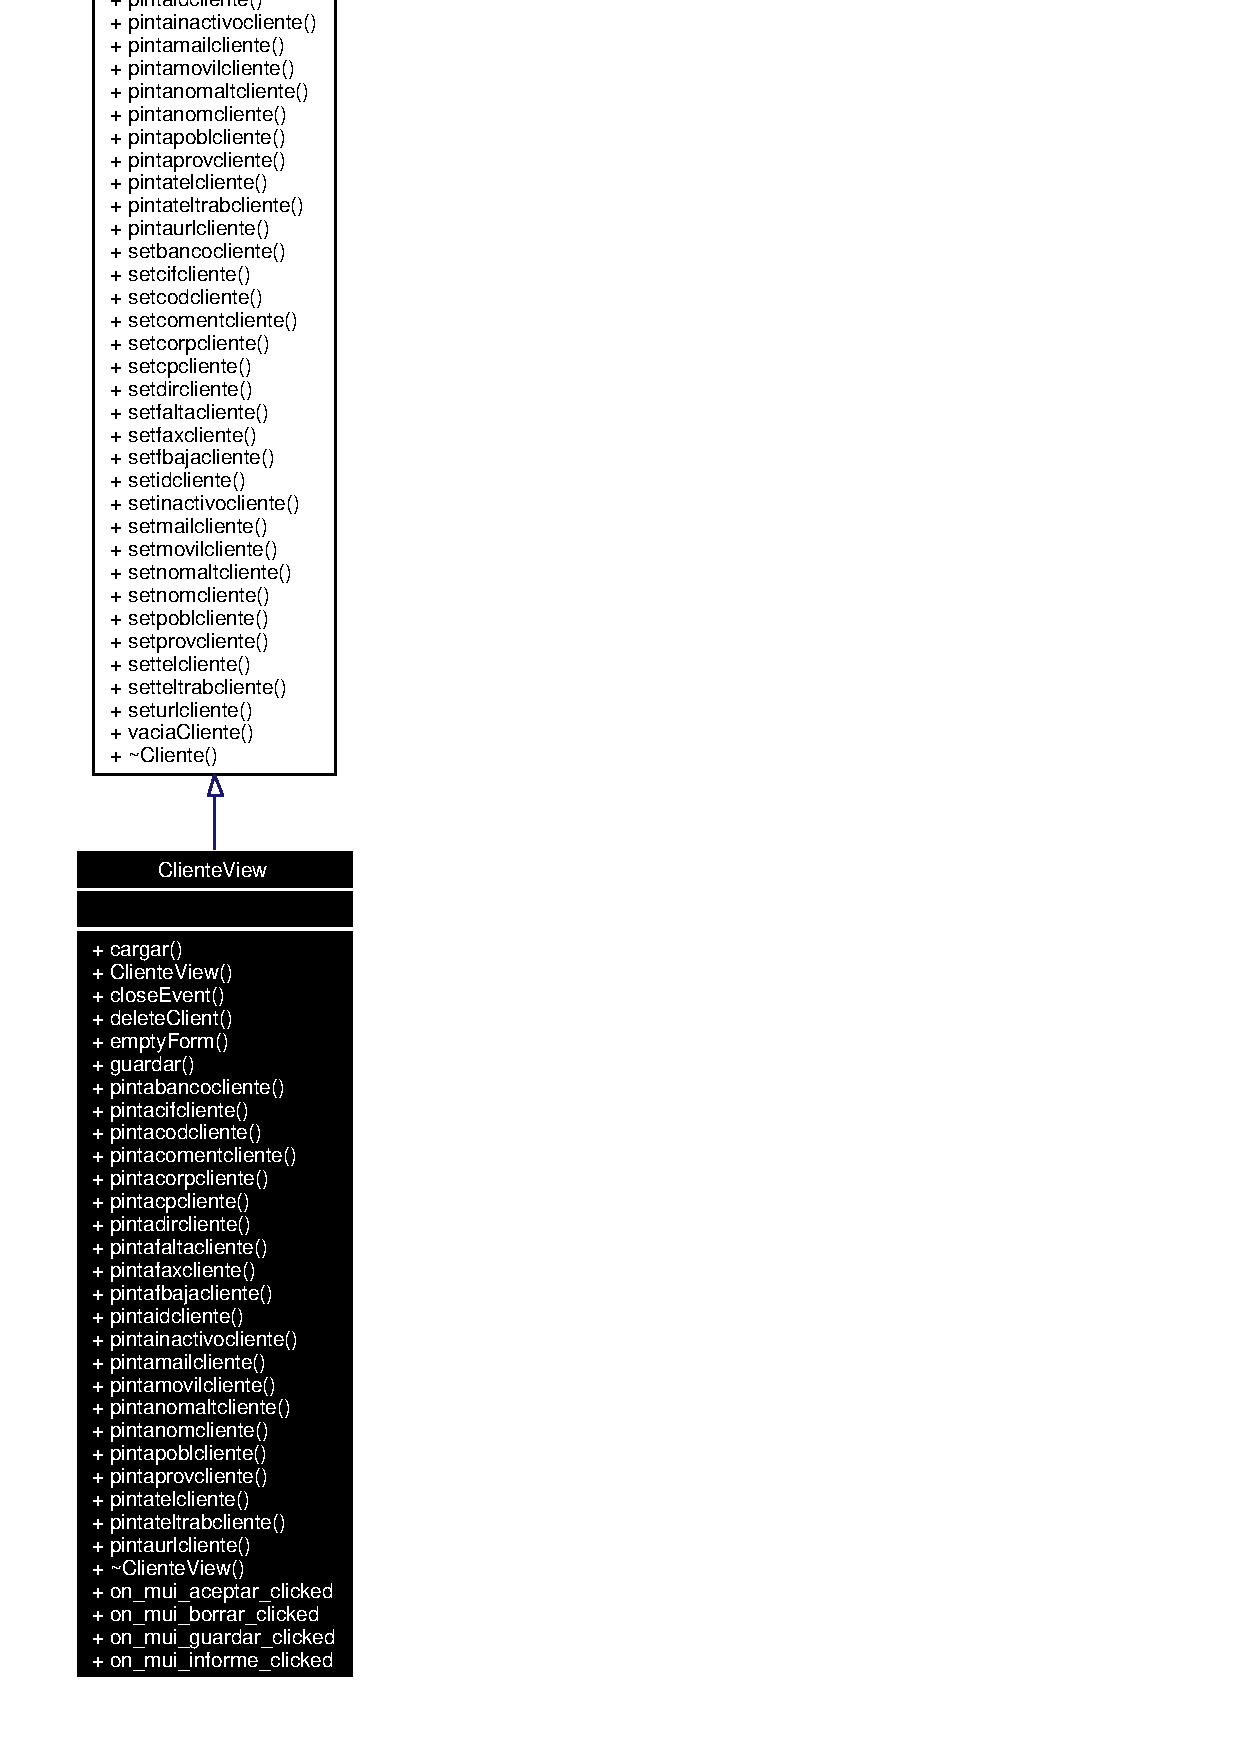
\includegraphics[width=85pt]{classClienteView__inherit__graph}
\end{center}
\end{figure}
Diagrama de colaboraci\'{o}n para Cliente\-View:\begin{figure}[H]
\begin{center}
\leavevmode
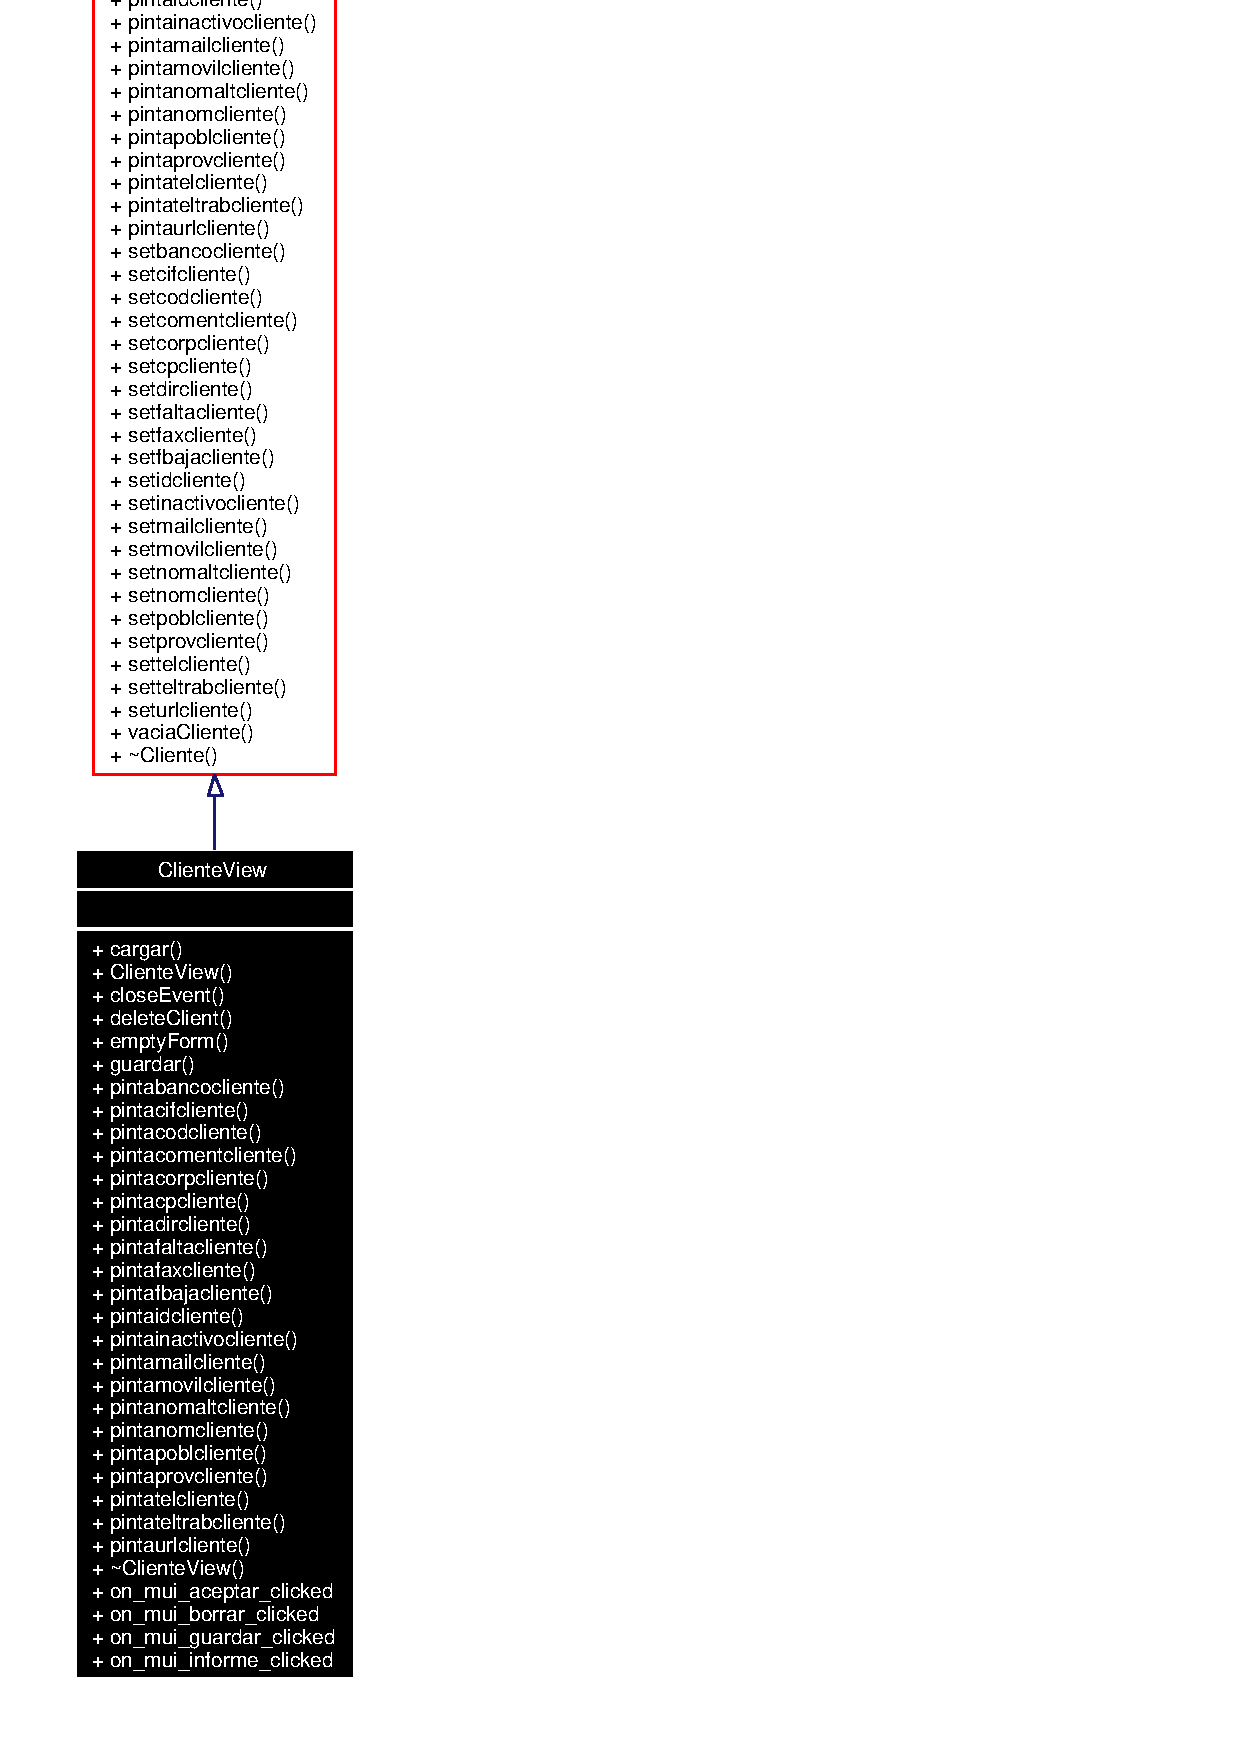
\includegraphics[width=85pt]{classClienteView__coll__graph}
\end{center}
\end{figure}
\subsection*{Slots p\'{u}blicos}
\begin{CompactItemize}
\item 
virtual void {\bf on\_\-mui\_\-aceptar\_\-clicked} ()\label{classClienteView_i0}

\item 
virtual void {\bf on\_\-mui\_\-borrar\_\-clicked} ()\label{classClienteView_i1}

\item 
virtual void {\bf on\_\-mui\_\-guardar\_\-clicked} ()\label{classClienteView_i2}

\item 
virtual void {\bf on\_\-mui\_\-informe\_\-clicked} ()\label{classClienteView_i3}

\end{CompactItemize}
\subsection*{M\'{e}todos p\'{u}blicos}
\begin{CompactItemize}
\item 
int {\bf cargar} (QString client)
\item 
{\bf Cliente\-View} ({\bf company} $\ast$emp, QWidget $\ast$parent=0)
\item 
void {\bf close\-Event} (QClose\-Event $\ast$)\label{classClienteView_a2}

\item 
void {\bf delete\-Client} ()
\item 
void {\bf empty\-Form} ()\label{classClienteView_a4}

\begin{CompactList}\small\item\em Empties the form. \item\end{CompactList}\item 
virtual int {\bf guardar} ()
\item 
void {\bf pintabancocliente} (QString val)\label{classClienteView_a6}

\item 
void {\bf pintacifcliente} (QString val)\label{classClienteView_a7}

\item 
void {\bf pintacodcliente} (QString val)\label{classClienteView_a8}

\item 
void {\bf pintacomentcliente} (QString val)\label{classClienteView_a9}

\item 
void {\bf pintacorpcliente} (QString val)\label{classClienteView_a10}

\item 
void {\bf pintacpcliente} (QString val)\label{classClienteView_a11}

\item 
void {\bf pintadircliente} (QString val)\label{classClienteView_a12}

\item 
void {\bf pintafaltacliente} (QString)\label{classClienteView_a13}

\item 
void {\bf pintafaxcliente} (QString val)\label{classClienteView_a14}

\item 
void {\bf pintafbajacliente} (QString)\label{classClienteView_a15}

\item 
void {\bf pintaidcliente} (QString)\label{classClienteView_a16}

\item 
void {\bf pintainactivocliente} (QString)\label{classClienteView_a17}

\item 
void {\bf pintamailcliente} (QString val)\label{classClienteView_a18}

\item 
void {\bf pintamovilcliente} (QString val)\label{classClienteView_a19}

\item 
void {\bf pintanomaltcliente} (QString val)\label{classClienteView_a20}

\item 
void {\bf pintanomcliente} (QString val)\label{classClienteView_a21}

\item 
void {\bf pintapoblcliente} (QString val)\label{classClienteView_a22}

\item 
void {\bf pintaprovcliente} (QString val)\label{classClienteView_a23}

\item 
void {\bf pintatelcliente} (QString val)\label{classClienteView_a24}

\item 
void {\bf pintateltrabcliente} (QString val)\label{classClienteView_a25}

\item 
void {\bf pintaurlcliente} (QString val)\label{classClienteView_a26}

\item 
{\bf $\sim$Cliente\-View} ()
\end{CompactItemize}


\subsection{Descripci\'{o}n detallada}
Muestra la ficha de un cliente. 



\subsection{Documentaci\'{o}n del constructor y destructor}
\index{ClienteView@{Cliente\-View}!ClienteView@{ClienteView}}
\index{ClienteView@{ClienteView}!ClienteView@{Cliente\-View}}
\subsubsection{\setlength{\rightskip}{0pt plus 5cm}Cliente\-View::Cliente\-View ({\bf company} $\ast$ {\em comp}, QWidget $\ast$ {\em parent} = {\tt 0})}\label{classClienteView_a1}


Disparamos los plugins.

Desabilitamos los tabs que aun no se usan.

Inicializamos las pantallas auxiliares a esta.

Disparamos los plugins. \index{ClienteView@{Cliente\-View}!~ClienteView@{$\sim$ClienteView}}
\index{~ClienteView@{$\sim$ClienteView}!ClienteView@{Cliente\-View}}
\subsubsection{\setlength{\rightskip}{0pt plus 5cm}Cliente\-View::$\sim$Cliente\-View ()}\label{classClienteView_a27}


Disparamos los plugins. 

\subsection{Documentaci\'{o}n de las funciones miembro}
\index{ClienteView@{Cliente\-View}!cargar@{cargar}}
\index{cargar@{cargar}!ClienteView@{Cliente\-View}}
\subsubsection{\setlength{\rightskip}{0pt plus 5cm}int Cliente\-View::cargar (QString {\em idcliente})\hspace{0.3cm}{\tt  [virtual]}}\label{classClienteView_a0}


load\-Client

Given a valid client ID this function loads the client into the form so that we can edit it.

Otherwise it empties the form and sets it so that we can add a new client

Hacemos que el listado de presupuestos de un cliente se inicialize. 

Reimplementado de {\bf Cliente} {\rm (p.\,\pageref{classCliente_a1})}.\index{ClienteView@{Cliente\-View}!deleteClient@{deleteClient}}
\index{deleteClient@{deleteClient}!ClienteView@{Cliente\-View}}
\subsubsection{\setlength{\rightskip}{0pt plus 5cm}void Cliente\-View::delete\-Client ()}\label{classClienteView_a3}


For now this function cleans the form and sets it so that we can add a new client

In the future it should really delete the client, or better yet mark it as deleted on an appropiate field in the DB\index{ClienteView@{Cliente\-View}!guardar@{guardar}}
\index{guardar@{guardar}!ClienteView@{Cliente\-View}}
\subsubsection{\setlength{\rightskip}{0pt plus 5cm}int Cliente\-View::guardar ()\hspace{0.3cm}{\tt  [virtual]}}\label{classClienteView_a5}


save\-Client

This function saves the current client. It checks if it is a new client that needs to be added or if it is an existing one that has to be modified

Disparamos los plugins con presupuesto\_\-imprimir\-Presupuesto. 

Reimplementado de {\bf Cliente} {\rm (p.\,\pageref{classCliente})}.

La documentaci\'{o}n para esta clase fu\'{e} generada a partir de los siguientes archivos:\begin{CompactItemize}
\item 
clienteview.h\item 
clienteview.cpp\end{CompactItemize}
